\documentclass[12pt]{beamer}
\usepackage{listings}
\usepackage{color}
\usepackage{xcolor}
%\usepackage{latexsym}
\usepackage{amsmath}
\usepackage[labelfont=bf]{caption}
\usepackage{graphicx}  %package graphic
\usepackage{siunitx}
\usepackage{tikz}
%\usepackage{algorithmicx}
%\usepackage[noend]{algpseudocode}
\usetikzlibrary{automata, positioning, arrows}
\usetheme{Boadilla}   
\usepackage{xeCJK}
%\usepackage{array}
%\usepackage{tabularx}
%\usepackage{mathtools}
\usepackage{listings}
%\usepackage{textcomp}
\usepackage[T1]{fontenc}
\usepackage{lmodern}
\usepackage{adjustbox}
\usepackage{dirtree}
\usepackage{hyperref}
\usepackage{inconsolata}

\setCJKmainfont{微軟正黑體} 
\sisetup{
	group-separator={,},
	table-number-alignment=right
}


\setbeamerfont{title}{size=\Large,series=\bfseries}  % title size

\setbeamerfont{frametitle}{size=\large,series=\bfseries}  % frametitle size, also can size*=<pt>

\definecolor{themeColor}{rgb}{0.06, 0.3, 0.57}
\usecolortheme[named=themeColor]{structure}

\defbeamertemplate*{footline}{Dan P theme}
{
  \leavevmode%
  \hbox{%
  %\begin{beamercolorbox}[wd=.2\paperwidth,ht=2.25ex,dp=1ex,center]{author in head/foot}%
	%\usebeamerfont{author in head/foot}\insertshortauthor\expandafter\beamer@ifempty\expandafter{\beamer@shortinstitute}{}{~~(\insertshortinstitute)}
  %\end{beamercolorbox}%
  \begin{beamercolorbox}[wd=.7\paperwidth,ht=2.25ex,dp=1ex,center]{title in head/foot}%
	\usebeamerfont{title in head/foot}\insertshorttitle
  \end{beamercolorbox}%
  \begin{beamercolorbox}[wd=.3\paperwidth,ht=2.25ex,dp=1ex,right]{date in head/foot}%
	\usebeamerfont{date in head/foot}\insertshortdate{}\hspace*{2em}
\insertframenumber{} / \inserttotalframenumber\hspace*{2ex} 
  \end{beamercolorbox}}%
  \vskip0pt%
}
\makeatother

% Item include picture
\setbeamertemplate{itemize item}   % First Level item
{
\includegraphics[height=0.33cm]{../Figures/golden-earth-on-white}}

\setbeamertemplate{itemize subitem} % Second level item
{
\includegraphics[height=0.31cm]{../Figures/golden-sun-on-white}}

\setbeamertemplate{itemize subsubitem} % Third Level item
{
\includegraphics[height=0.27cm]{../Figures/golden-paw-on-white}}

\definecolor{darkgold}{rgb}{0.765 0.64 0.0} % for highlighted text in black-and-white slides
\newcommand{\code}[1]{\texttt{#1}}

%\newtheorem{problem}{Problem}
\mode<presentation>{\newtheorem{algorithm}{Algorithm}}
\mode<article>{\newenvironment{algorithm}{}{}}
%\newtheorem{solution}{Solution}

\newlength{\subtextwidth}
\setlength{\subtextwidth}{11cm}

\newenvironment{cbox}{
	\begin{center}
	\begin{tabular}{|l|}
	\hline
	\begin{minipage}[t]{\subtextwidth}}
	{\vspace{.25ex}
	\end{minipage}
	\hline
	\end{tabular}
	\end{center} }

\lstdefinestyle{mystyle}{
	basicstyle=\setmonofont{Consolas},
	columns=fullflexible,
	keepspaces=true,
	upquote=true,
	showstringspaces=false,
	commentstyle=\color{gray},
	keywordstyle=\color{teal},
	identifierstyle=\color{black},
	stringstyle=\color{brown},
	language=C++
}

\lstset{style=mystyle,frame=single,}
\makeatletter
\lst@CCPutMacro
	\lst@ProcessOther {"2A}{%
	%   \lst@ttfamily 
		 {\raisebox{1.5pt}{*}}% used with ttfamily
		%   \textasteriskcentered
		  }% used with other fonts
	\@empty\z@\@empty
\makeatother


\newcommand{\mathdef}[1]{\relax\ifmmode #1\else $#1$\fi}
\newcommand{\true}{\mathdef{\mathit{true}}}
\newcommand{\false}{\mathdef{\mathit{false}}}
\renewcommand{\implies}{\mathdef{\rightarrow}}
\newcommand{\ifonlyif}{\mathdef{\leftrightarrow}}
\newcommand{\entails}{\mathdef{\vdash}}
\newcommand{\PROPS}{\mathdef{\mathit{PROPS}}}
\newcommand{\BOOL}{\mathdef{\mathit{BOOL}}}
\newcommand{\Note}[1]{\textsl{\small(#1)}}

\newcommand{\ultimate}{\textsc{Ultimate }}

\mode<presentation>{\title{Introduction to Utimate}}
\mode<article>{\title{Algorithms 2019: Analysis of Algorithms}}
\subtitle{(Based on [Daniel Dietsch : Automated verification of system requirements and software specifications. 2016.])}
\author{林宏陽}
%\institute[IM.NTU]{Department of Information Management\\ National Taiwan University}
%\date[Algorithms 2019]{\null}
\mode<presentation>{\date[SVVRL]{\null}}
\mode<article>{\date{\today}}

\begin{document}
\begin{frame}
	\maketitle
\end{frame}

\begin{frame}{Ultimate}
  	\begin{itemize}
		\item \ultimate is a modular, plugin-based program analysis framework. It provides a platform for the development of automated program analysis methods that facilitates the reuse of existing components (plugins) and analysis results.
		\item Website : \url{https://monteverdi.informatik.uni-freiburg.de/tomcat/Website/}
		\item Github page : \url{https://github.com/ultimate-pa/ultimate}
	  	\item Installation : Just follow the wiki page on github. \Note{Z3.exe should be updated in Windows.}
	\end{itemize}
\end{frame}

\begin{frame}{Core Architecture and Plugin Lifecycles}
  	\begin{itemize}
		\item The \ultimate framework is based on the Eclipse Rich Client Platform
	(Eclipse RCP).
		\item Eclipse RCP is a software development framework that provides  the ability to load and unload plugins dynamically at runtime and isolate them from each other.
		\item Eclipse RCP is written in the programming language Java.
		Hence, most of \ultimate is also written in Java (currently, Java 11).
  	\end{itemize}
\end{frame}

\begin{frame}{Core Architecture and Plugin Lifecycles (cont'd)}
	\begin{itemize}
	  	\item  In this context, the plugin \code{UltimateCore} provides the interface between Eclipse RCP and all active plugins.
	  	\item  Plugins can be executed one after another in a \textbf{toolchain}. A toolchain is defined by an XML file.
	  	\item \code{UltimateCore} manages different representations of a program analysis problem as models and passes them between active plugins according to the toolchain. The plugins may analyse, transform, or visualize the models they receive.
	\end{itemize}
\end{frame}

\captionsetup[figure]{font=scriptsize ,labelfont=scriptsize}
\begin{frame}{Ultimate toolchain illustration}
    \begin{figure}
        \centering
        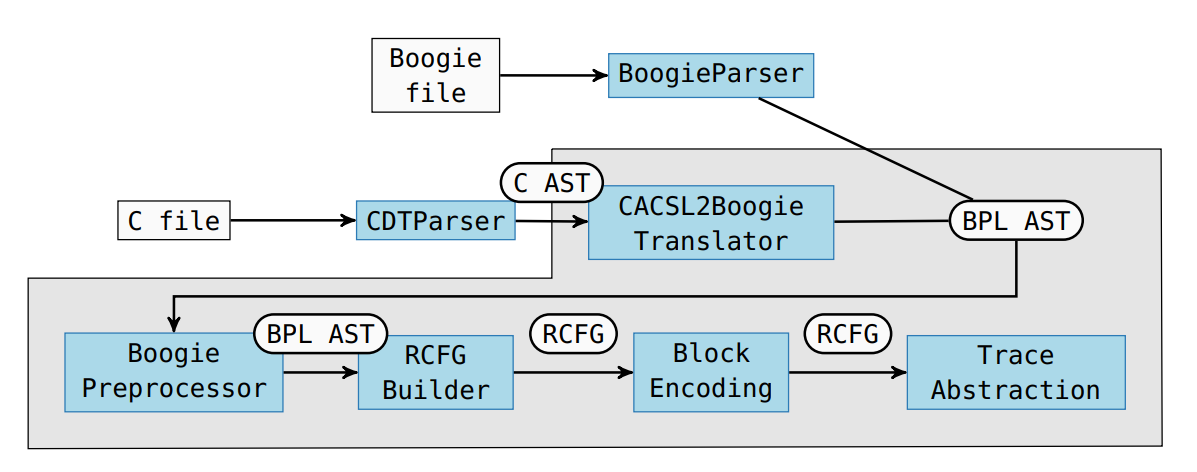
\includegraphics[scale=0.35]{toolchain.png}
        \caption{\ultimate toolchain for the tool ultimate \textsc{Automizer}. The light boxes are input files, the dark boxes are plugins, the rounded boxes are the internal models that are passed between the plugins, and the shaded area is the toolchain for C programs. Removing the plugin \code{CACSL2BoogieTranslator} from the toolchain defines a new toolchain that can be used to process Boogie programs.
		}
    \end{figure}    
\end{frame}

\begin{frame}{Reference}
	\begin{itemize}
		\item Ultimate website\\
		\url{https://monteverdi.informatik.uni-freiburg.de/tomcat/Website/}
		\item Daniel Dietsch : Automated verification of system requirements and software specifications. 2016.\\
		\url{https://freidok.uni-freiburg.de/data/11159}
	\end{itemize}
\end{frame}


\end{document}